%!TEX root = main.tex


\section{$p_\mathrm{T}^\mathrm{jet,ch}$ at $\sqrt{s}$ = 8 TeV}

\begin{frame}
\frametitle{Data samples}
ALICE data
\begin{table}[htp]
\begin{center}
\begin{tabular}{|c|c|c|c|c|}
\hline
Type & $\sqrt{s}$ & Period & Trigger & $\#$ of events\\
\hline
\multirow{ 2}{*}{pp} & \multirow{ 2}{*}{8} & \multirow{ 2}{*}{LHC12h} & INT7 & $29.3\times10^6$ \\
                    &                    &													& EMCEJE & $6.06\times10^6$ \\

\hline
\end{tabular}
\end{center}
\label{default}
\end{table}%

Monte Carlo
\begin{table}[htp]
\begin{center}
\begin{tabular}{|c|c|c|c|c|}
\hline
Type & $\sqrt{s}$ & Period & $\#$ of $p_\mathrm{T}$ hard bins & $\#$ of events\\
\hline
PYTHIA8 & 8 & LHC16c2 & 20 $^{[1]}$ & $28.1\times10^6$ \\
\hline
\end{tabular}
\end{center}
\label{default}
\end{table}%
\footnotetext[1] {5-7-9-12-16-21-28-36-45-57-70-85-99-115-132-150-169-190-212-235- GeV/$c$}

\end{frame}


\begin{frame}
\frametitle{$p_\mathrm{T}$ hard-bin normalization}
Steps
\begin{itemize}
\item{Follows the official procedure $^{[1]}$}
\item{Weighted by $\sigma$/ntirals given by MC header per event}
\item{Each hard-bin merged separately}
\item{Then divided by $\#$ of filled events for the given hard bin}
\item{Finally all hard bins are merged}
\item{Observables have the unit, mb \\(normalised to the cross-section)}
\end{itemize}
\scriptsize
\footnotetext[1]{https://twiki.cern.ch/twiki/bin/view/ALICE/PPEventNormalisation}
\end{frame}

\begin{frame}
\frametitle{Corrections}
$\frac{1}{N_\mathrm{evt}^\mathrm{EMCEJE}} \frac{\mathrm{d}N}{\mathrm{d}p_\mathrm{T,raw}^\mathrm{jet,ch}}$ is corrected by
\begin{itemize}
\item{EMCEJE to INT7 trigger efficiency\\
\small
$\frac{1}{N_\mathrm{evt}^\mathrm{EMCEJE}} \frac{\mathrm{d}N}{\mathrm{d}p_\mathrm{T,raw}^\mathrm{jet,ch}}$
$\times$ $\frac{\frac{1}{N_\mathrm{evt}^\mathrm{INT7}} \frac{\mathrm{d}N}{\mathrm{d}p_\mathrm{T,raw}^\mathrm{jet,ch}}}{\frac{1}{N_\mathrm{evt}^\mathrm{EMCEJE}} \frac{\mathrm{d}N}{\mathrm{d}p_\mathrm{T,raw}^\mathrm{jet,ch}}}$
\normalsize}
\item{Detector and vertex efficiency correction by the unfolding
\small
$\frac{1}{N_\mathrm{evt}^\mathrm{EMCEJE}} \frac{\mathrm{d}N}{\mathrm{d}p_\mathrm{T,raw}^\mathrm{jet,ch}}$
$\times$ $\frac{\frac{1}{N_\mathrm{evt}^\mathrm{INT7}} \frac{\mathrm{d}N}{\mathrm{d}p_\mathrm{T,raw}^\mathrm{jet,ch}}}{\frac{1}{N_\mathrm{evt}^\mathrm{EMCEJE}} \frac{\mathrm{d}N}{\mathrm{d}p_\mathrm{T,raw}^\mathrm{jet,ch}}}$
$\times$ $\mathcal{R}^{-1}(\frac{1}{N_\mathrm{evt}^\mathrm{mcrec}} \frac{\mathrm{d}N}{\mathrm{d}p_\mathrm{T,mcrec}^\mathrm{jet,ch}},\frac{1}{N_\mathrm{evt}^\mathrm{mcgen}} \frac{\mathrm{d}N}{\mathrm{d}p_\mathrm{T,mcgen}^\mathrm{jet,ch}})$
}
\normalsize
\item{Cross-section scaling and INT7 to INEL trigger efficiency}
\begin{itemize}
	\item{Multiplied by cross-section scaling : 55.8 $\pm$ 1.2 mb $^{[1]}$}
	\item{Divided by trigger efficiency : 85 $\%$}
\end{itemize}

\end{itemize}
\footnotetext[1]{https://aliceinfo.cern.ch/Notes/node/531}
\end{frame}

\begin{frame}
\frametitle{EMCEJE to INT7 scaling}
\begin{columns}[c]
\column{.5\textwidth}
\centering
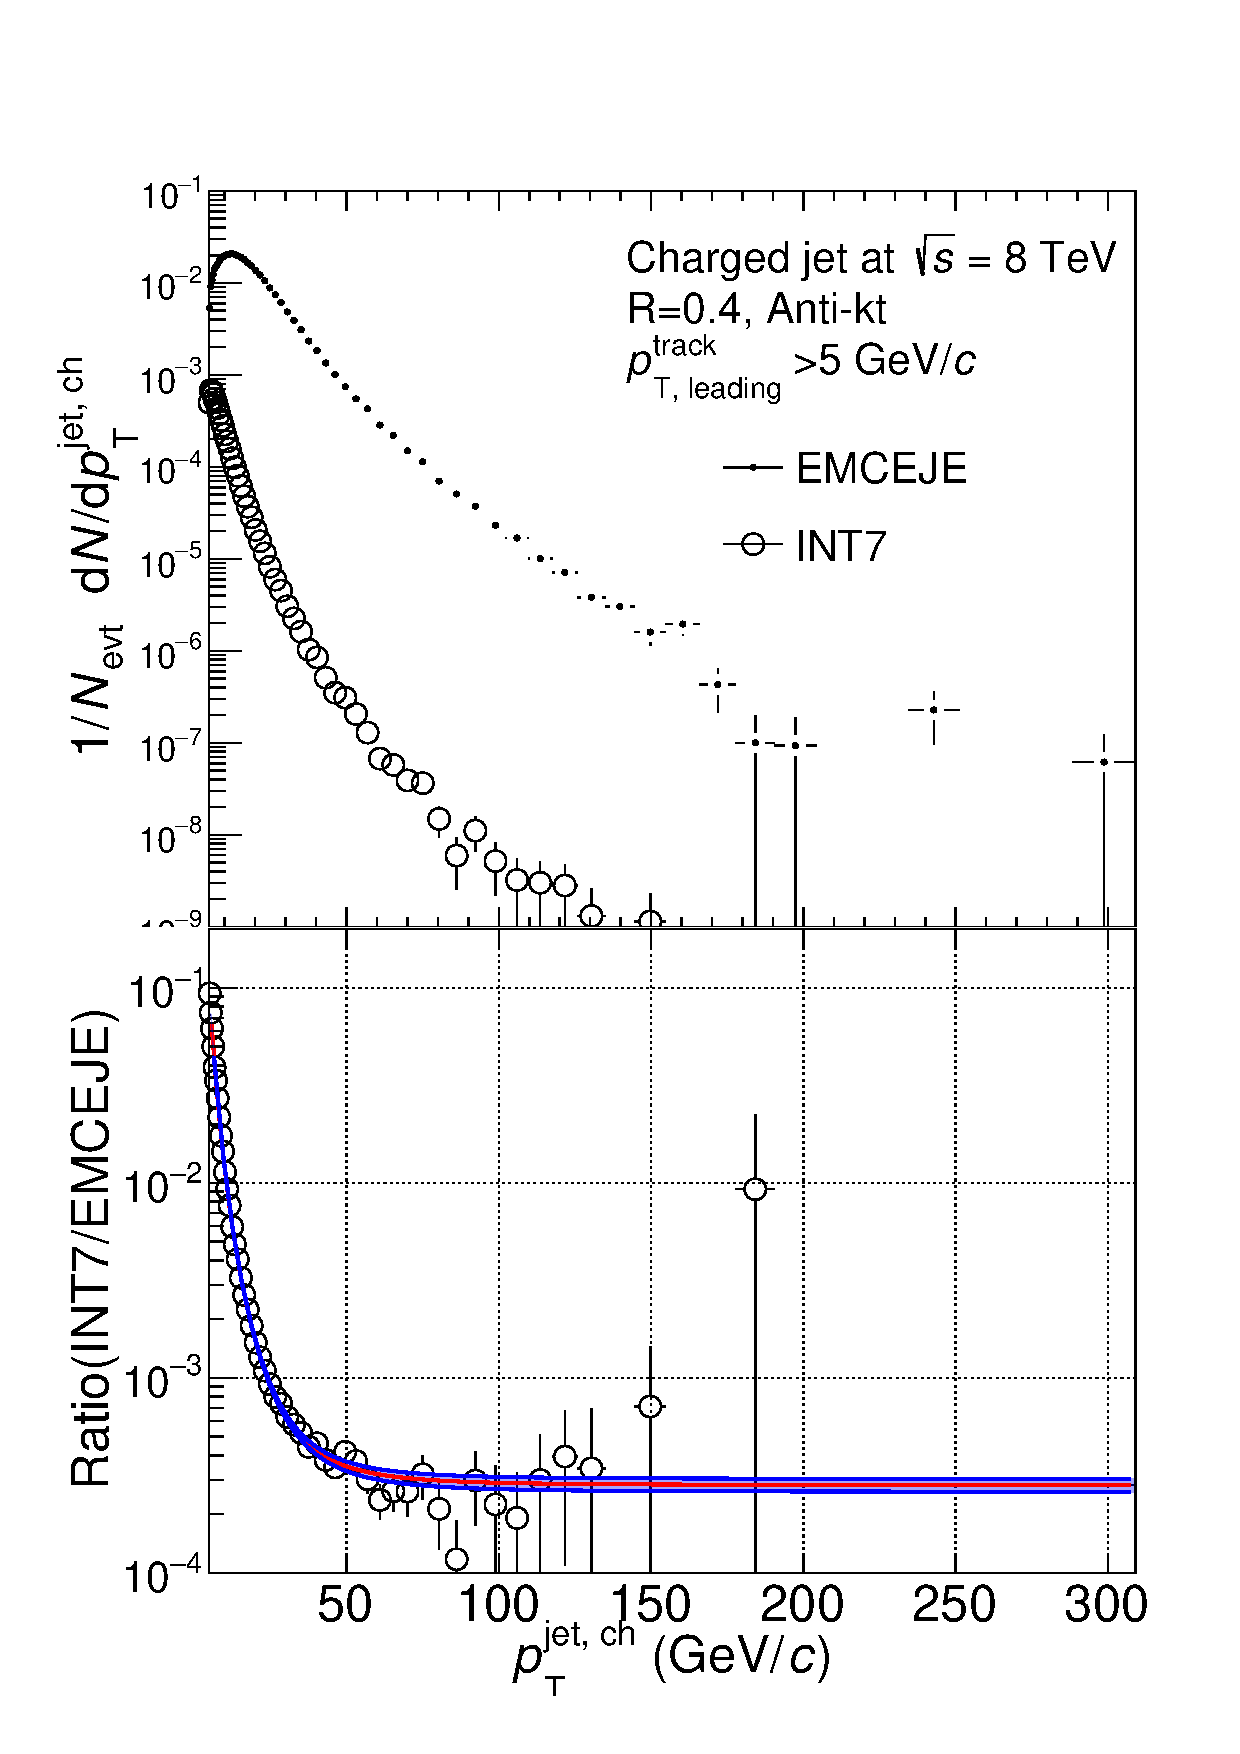
\includegraphics[width=1\linewidth]{JetToINT7TriggEff8TeV}\\
\column{.5\textwidth}
\begin{itemize}
  \item{Ratio shows \\ $\frac{\frac{1}{N_\mathrm{evt}^\mathrm{INT7}} \frac{\mathrm{d}N}{\mathrm{d}p_\mathrm{T,raw}^\mathrm{jet,ch}}}{\frac{1}{N_\mathrm{evt}^\mathrm{EMCEJE}} \frac{\mathrm{d}N}{\mathrm{d}p_\mathrm{T,raw}^\mathrm{jet,ch}}}$}
	\item{Fitted with $\frac{A}{(B+x^4)^C}+D$}
	\item{95 $\%$ confidence-range \\- Shown with blue\\- Systematic uncertainty}
  \item{Fit function\\- when on-the-fly filling}
\end{itemize}
\end{columns}
\end{frame}


\begin{frame}
\frametitle{Unfolding - closure test}
Detector efficiency is corrected by the unfolding method
\begin{columns}[c]
\column{.5\textwidth}
\centering
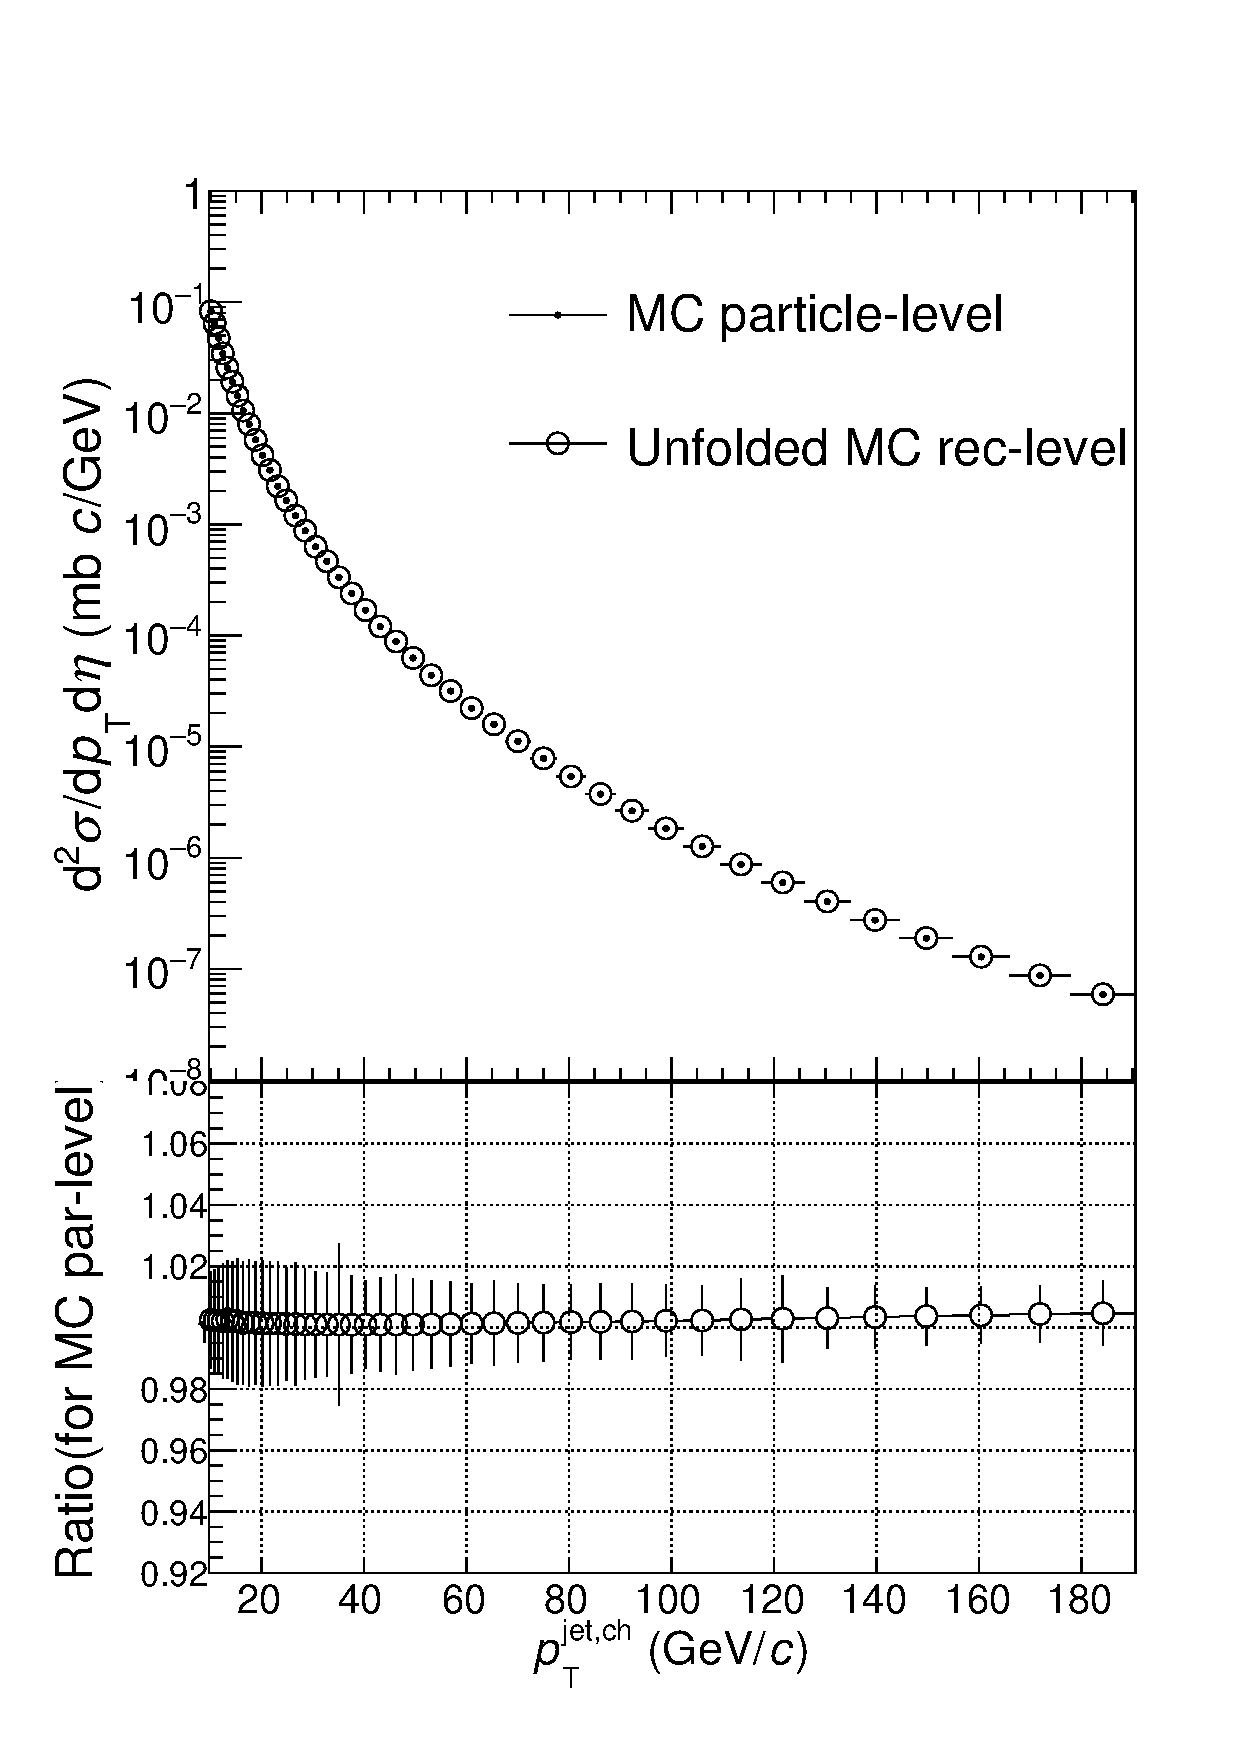
\includegraphics[width=1\linewidth]{jetpt_closure}\\
\column{.5\textwidth}
\begin{itemize}
  \small
	\item{Unfolding process\\$\frac{1}{N_\mathrm{evt}^\mathrm{EMCEJE}} \frac{\mathrm{d}N}{\mathrm{d}p_\mathrm{T,raw}^\mathrm{jet,ch}}$
  $\times$ $\frac{\frac{1}{N_\mathrm{evt}^\mathrm{INT7}} \frac{\mathrm{d}N}{\mathrm{d}p_\mathrm{T,raw}^\mathrm{jet,ch}}}{\frac{1}{N_\mathrm{evt}^\mathrm{EMCEJE}} \frac{\mathrm{d}N}{\mathrm{d}p_\mathrm{T,raw}^\mathrm{jet,ch}}}$
  \\ $\times$ $\mathcal{R}^{-1}(\frac{1}{N_\mathrm{evt}^\mathrm{mcrec}} \frac{\mathrm{d}N}{\mathrm{d}p_\mathrm{T,mcrec}^\mathrm{jet,ch}},\frac{1}{N_\mathrm{evt}^\mathrm{mcgen}} \frac{\mathrm{d}N}{\mathrm{d}p_\mathrm{T,mcgen}^\mathrm{jet,ch}})$}
  \normalsize
  \item{Package : RooUnfold}
	\item{Algorithm : Iterative(Bayesian)}
	\item{Regularization parameter : 4}
\end{itemize}
\end{columns}
\end{frame}


\begin{frame}
\frametitle{Final result}
\begin{columns}[c]
\column{.5\textwidth}
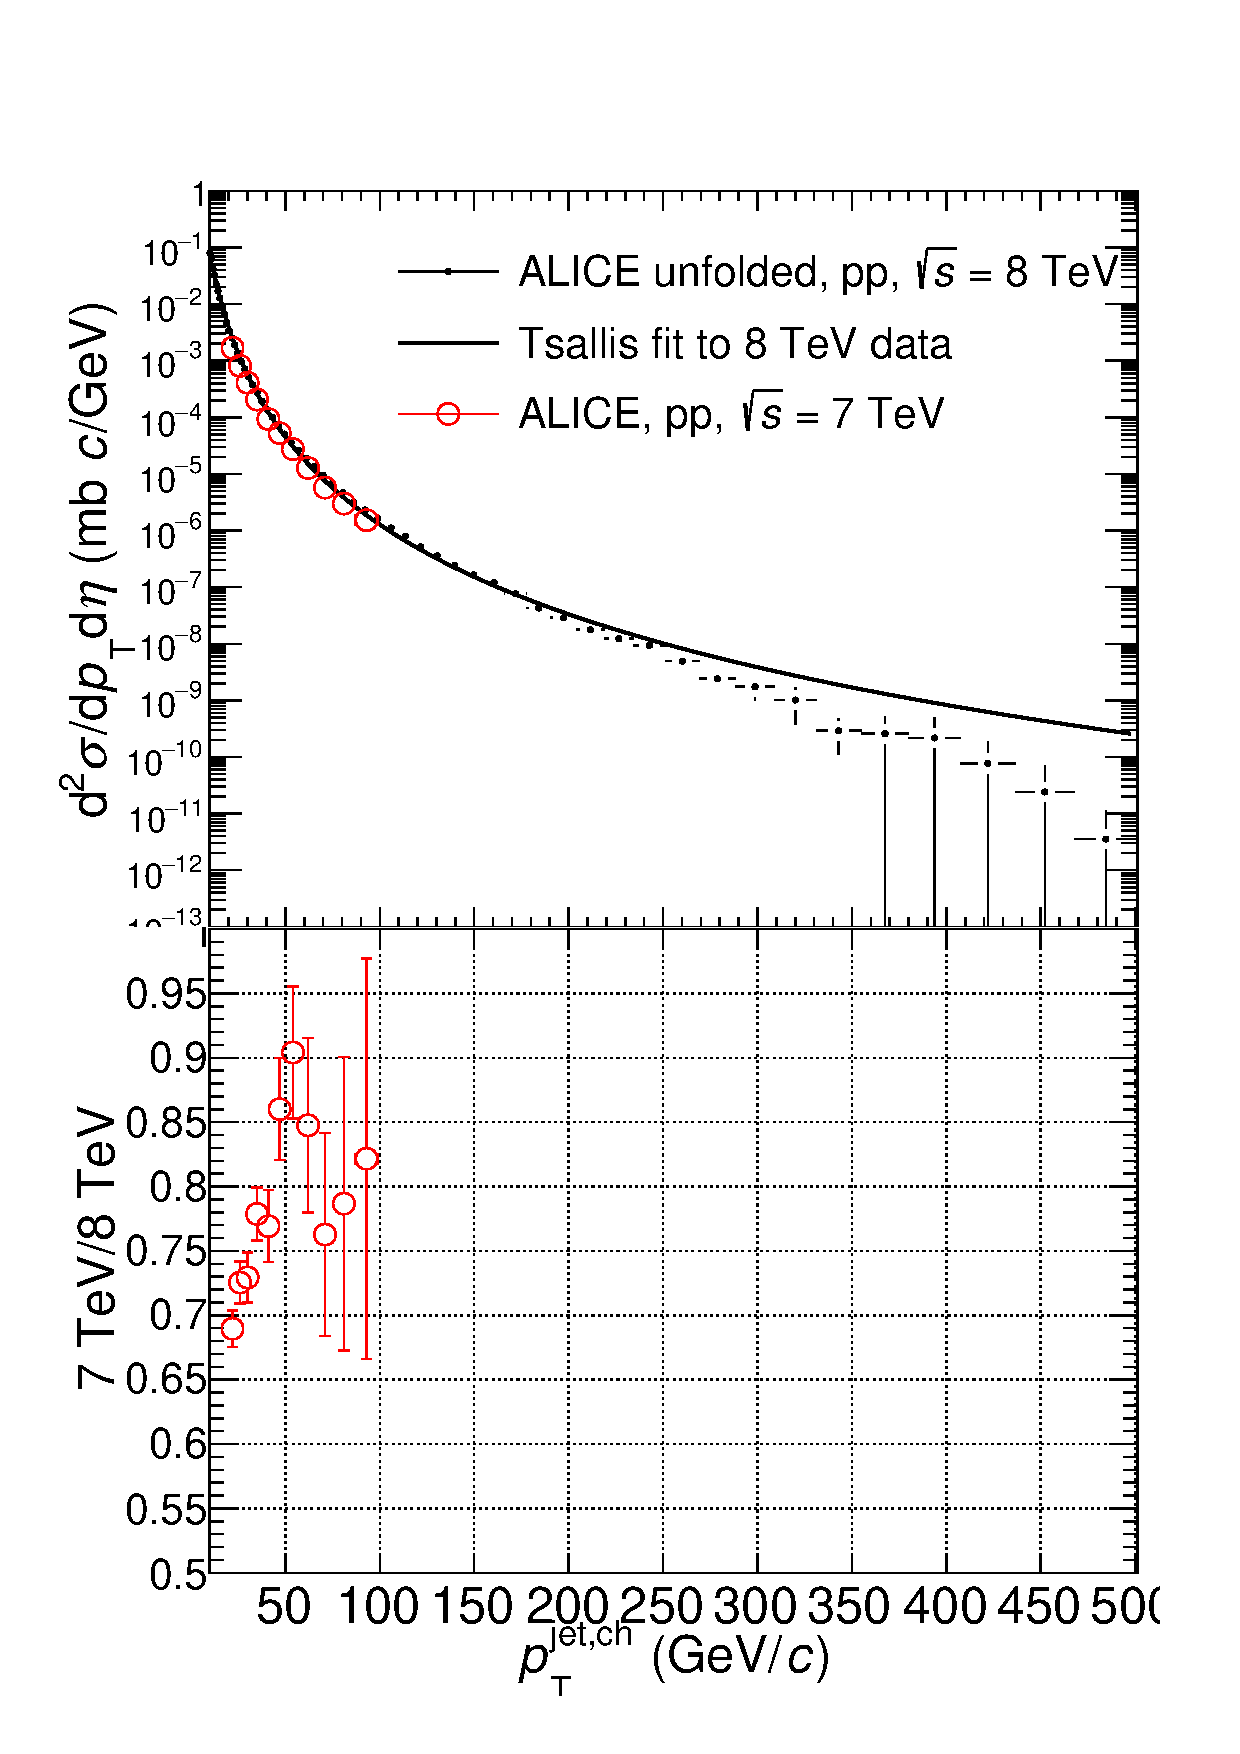
\includegraphics[width=1\linewidth]{jetpt_data_data.pdf}
\column{.5\textwidth}
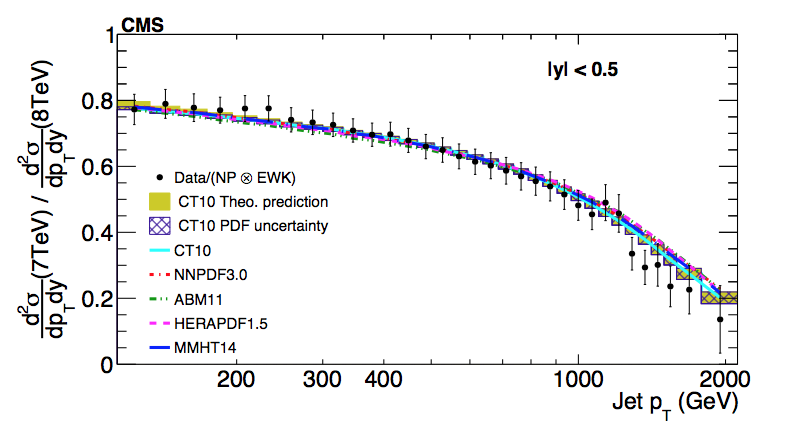
\includegraphics[width=1\linewidth]{CMSratio}\\
Ratio of CMS full jet spectra beteen 7 and 8 TeV$^{[1]}$
\begin{itemize}
  \item{around 0.8}
  \item{support the new 8 TeV result}
\end{itemize}
The new 8 TeV result extends to 300 GeV/$c$ (7 TeV, 100 GeV/$c$)
\end{columns}
\footnotetext[1]{arXiv:1609.05331v2 [hep-ex] 4 Apr 2017}
\end{frame}

\begin{frame}
\frametitle{Final result v.s models}
\begin{columns}[c]
\column{.5\textwidth}
\centering
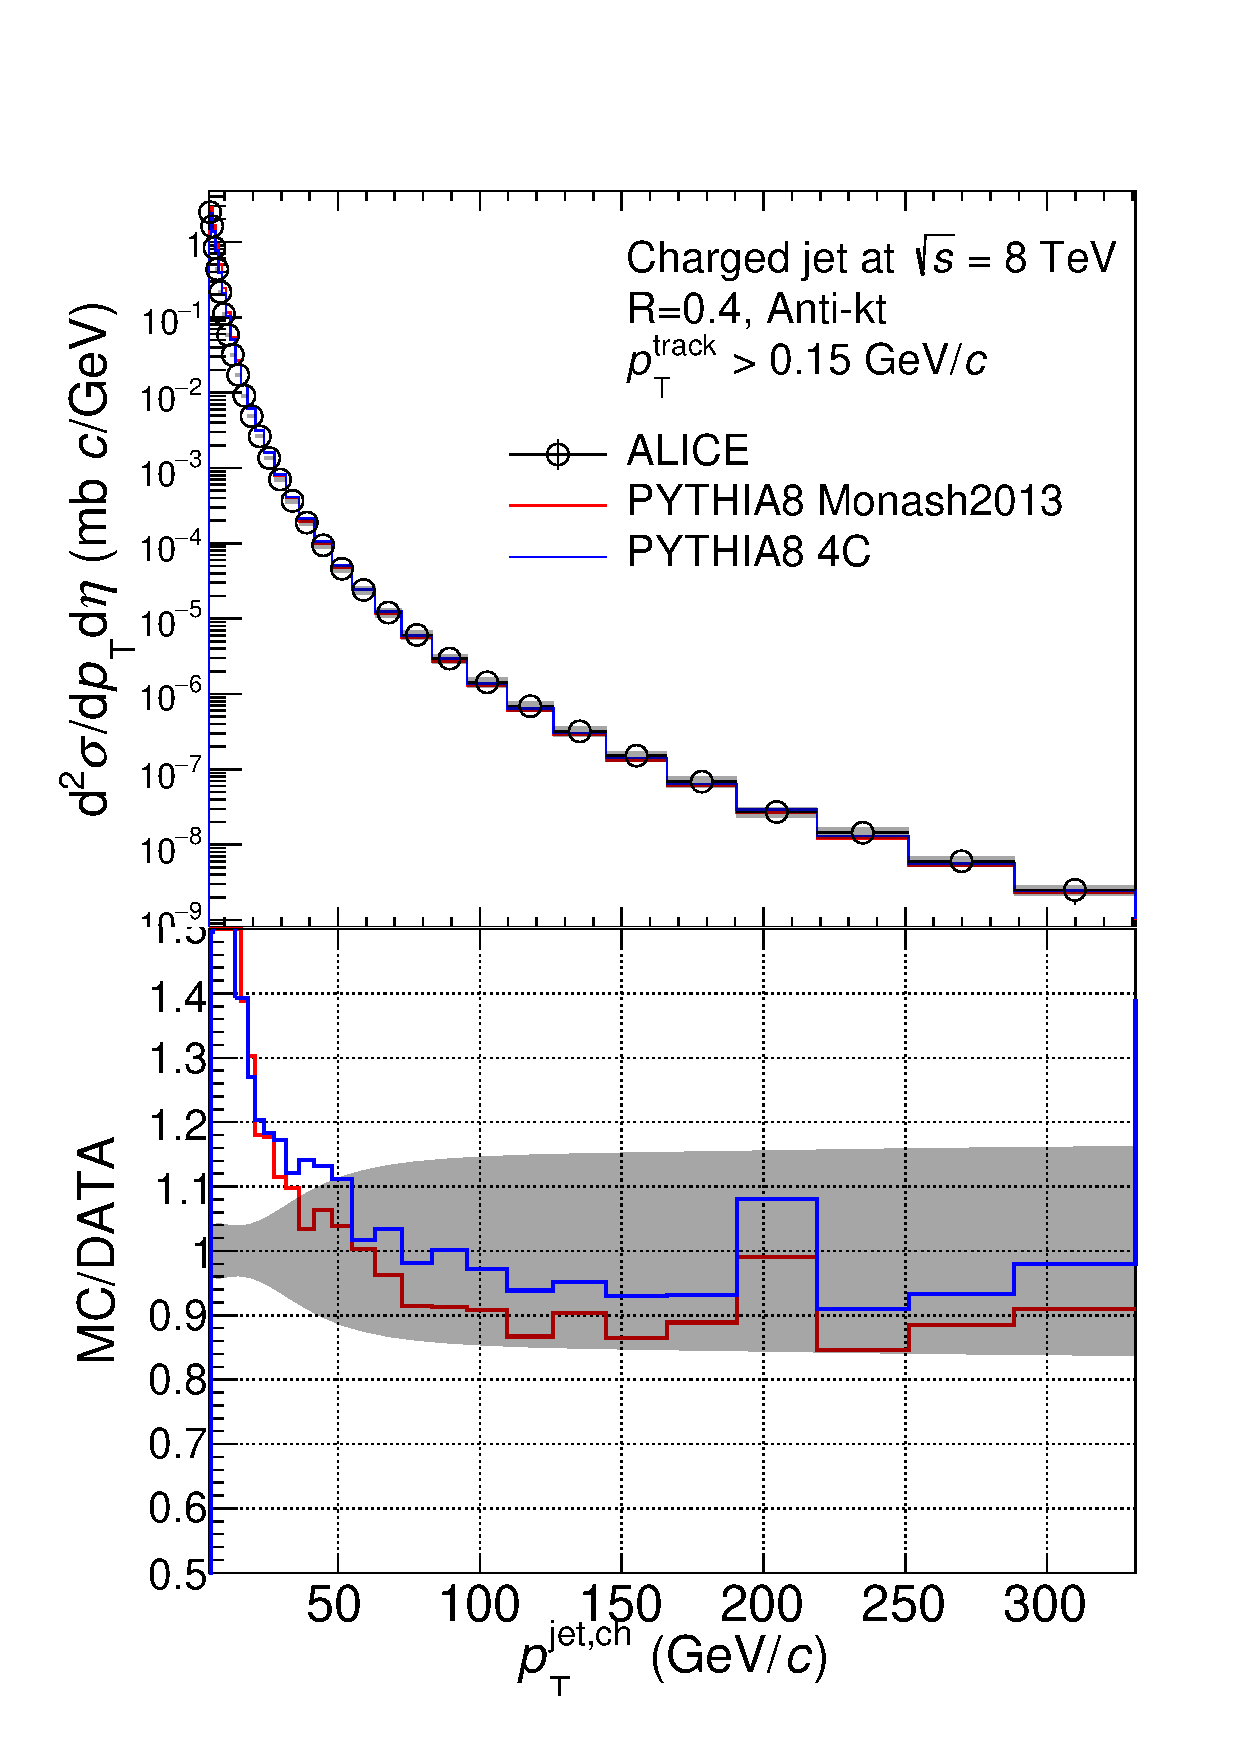
\includegraphics[width=1\linewidth]{jetpt8tev}\\
\column{.5\textwidth}
Systematic uncertainty
\begin{itemize}
  \item{Jet to INT7 trigger scaling : 10 $\%$}
  \item{INT7 to INEL normalisation : 2.95$\%$ \\(0.7718$\pm$0.0228 (2.95$\%$))}
  \item{Unfolding : 3 $\%$ }
\end{itemize}

\end{columns}
\end{frame}

%\begin{frame}
%\frametitle{Scaling to 5.02 TeV}
%pp results should be scaled to 5 TeV \\ to compare with 5 TeV p-Pb and Pb-Pb results
%\begin{columns}[t]
%\column{.5\textwidth}
%\centering
%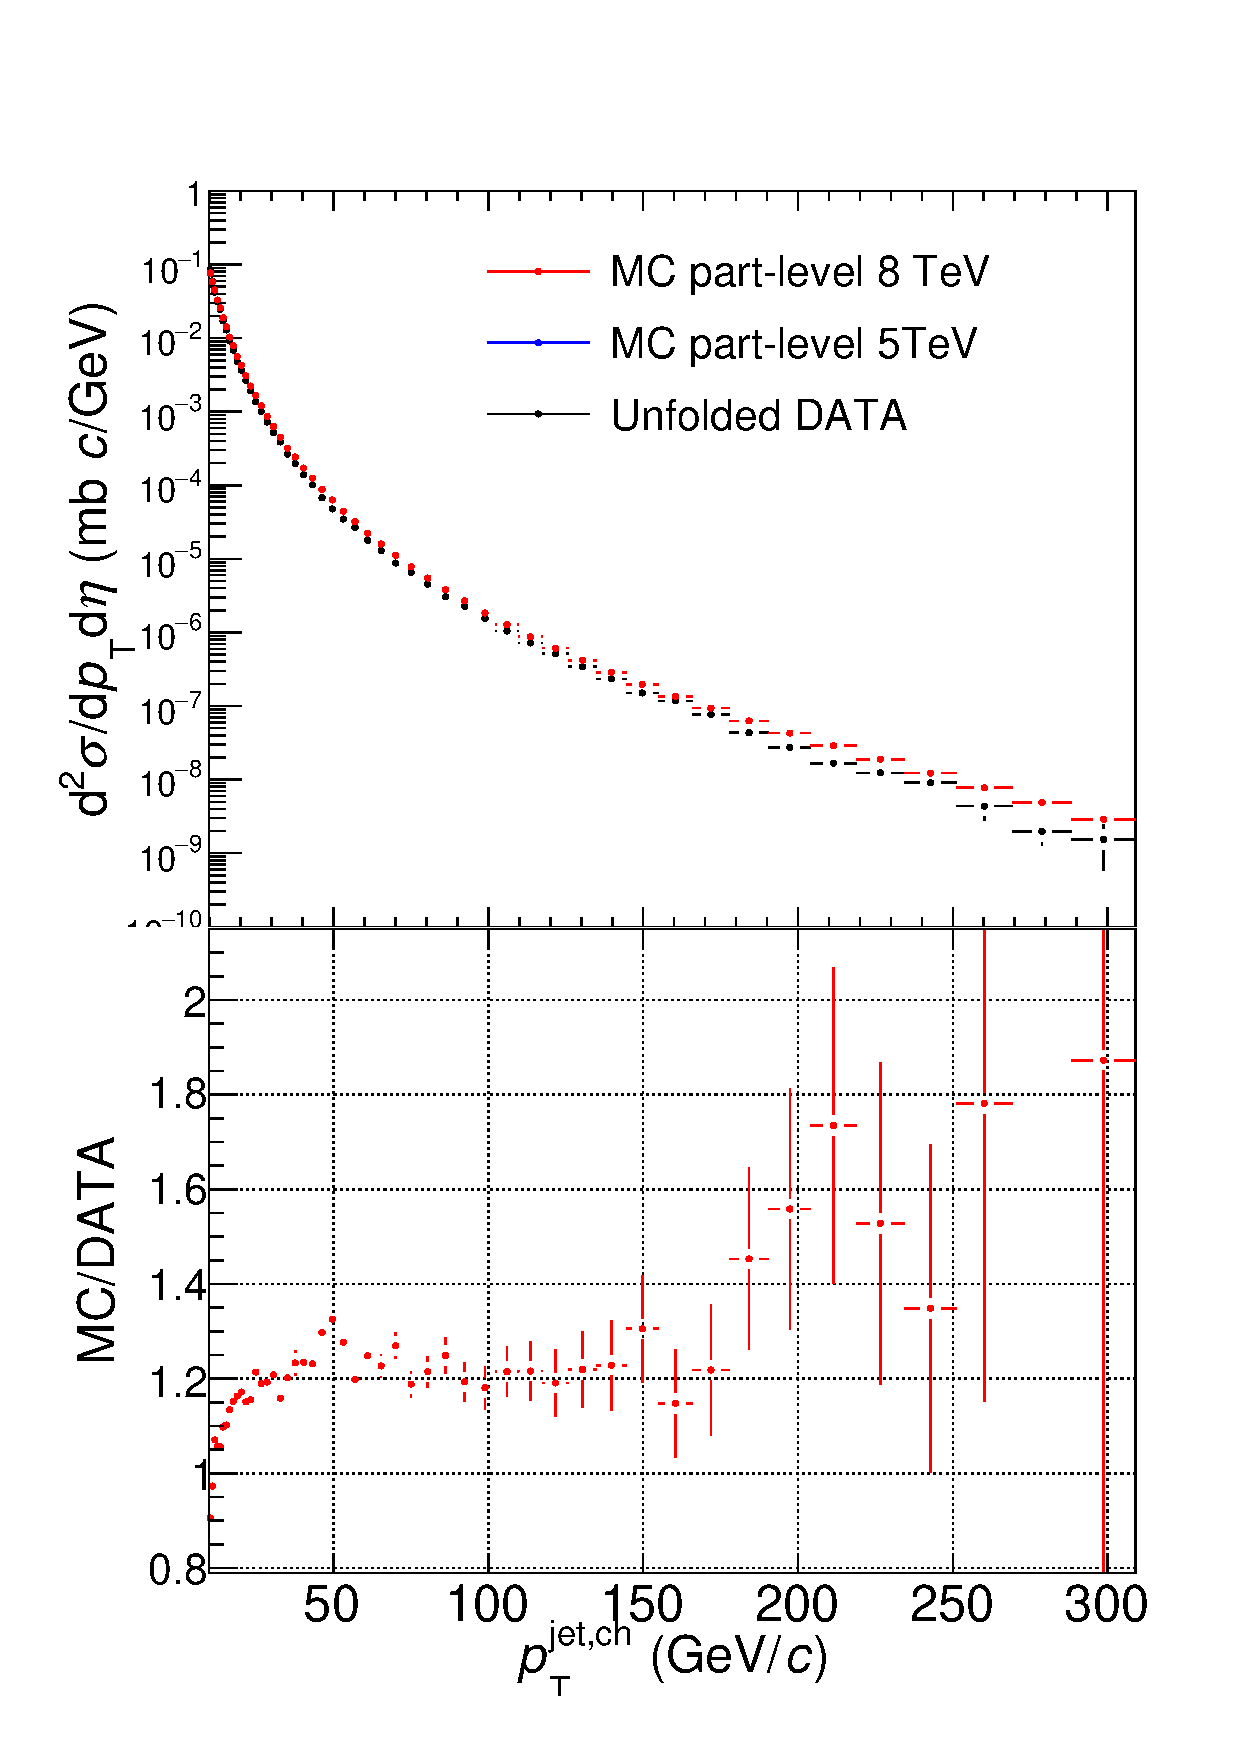
\includegraphics[width=1\linewidth]{jetpt_data_mc}\\
%\column{.5\textwidth}
%\end{columns}
%\end{frame}
%!TEX root = main.tex


\section{$p_\mathrm{T}^\mathrm{jet,ch}$ at $\sqrt{s}$ = 8 TeV}

\begin{frame}
\frametitle{Data samples}
ALICE data
\begin{table}[htp]
\begin{center}
\begin{tabular}{|c|c|c|c|c|}
\hline
Type & $\sqrt{s}$ & Period & Trigger & $\#$ of events\\
\hline
\multirow{ 2}{*}{pp} & \multirow{ 2}{*}{8} & \multirow{ 2}{*}{LHC12h} & INT7 & $29.3\times10^6$ \\
                    &                    &													& EMCEJE & $6.06\times10^6$ \\

\hline
\end{tabular}
\end{center}
\label{default}
\end{table}%

Monte Carlo
\begin{table}[htp]
\begin{center}
\begin{tabular}{|c|c|c|c|c|}
\hline
Type & $\sqrt{s}$ & Period & $\#$ of $p_\mathrm{T}$ hard bins & $\#$ of events\\
\hline
PYTHIA8 & 8 & LHC16c2 & 20 $^{[1]}$ & $28.1\times10^6$ \\
\hline
\end{tabular}
\end{center}
\label{default}
\end{table}%
\footnotetext[1] {5-7-9-12-16-21-28-36-45-57-70-85-99-115-132-150-169-190-212-235- GeV/$c$}

\end{frame}


\begin{frame}
\frametitle{$p_\mathrm{T}$ hard-bin normalization}
Steps
\begin{itemize}
\item{Follows the official procedure $^{[1]}$}
\item{Weighted by $\sigma$/ntirals given by MC header per event}
\item{Each hard-bin merged separately}
\item{Then divided by $\#$ of filled events for the given hard bin}
\item{Finally all hard bins are merged}
\item{Observables have the unit, mb \\(normalised to the cross-section)}
\end{itemize}
\scriptsize
\footnotetext[1]{https://twiki.cern.ch/twiki/bin/view/ALICE/PPEventNormalisation}
\end{frame}

\begin{frame}
\frametitle{Corrections}
$\frac{1}{N_\mathrm{evt}^\mathrm{EMCEJE}} \frac{\mathrm{d}N}{\mathrm{d}p_\mathrm{T,raw}^\mathrm{jet,ch}}$ is corrected by
\begin{itemize}
\item{EMCEJE to INT7 trigger efficiency\\
\small
$\frac{1}{N_\mathrm{evt}^\mathrm{EMCEJE}} \frac{\mathrm{d}N}{\mathrm{d}p_\mathrm{T,raw}^\mathrm{jet,ch}}$
$\times$ $\frac{\frac{1}{N_\mathrm{evt}^\mathrm{INT7}} \frac{\mathrm{d}N}{\mathrm{d}p_\mathrm{T,raw}^\mathrm{jet,ch}}}{\frac{1}{N_\mathrm{evt}^\mathrm{EMCEJE}} \frac{\mathrm{d}N}{\mathrm{d}p_\mathrm{T,raw}^\mathrm{jet,ch}}}$
\normalsize}
\item{Detector and vertex efficiency correction by the unfolding
\small
$\frac{1}{N_\mathrm{evt}^\mathrm{EMCEJE}} \frac{\mathrm{d}N}{\mathrm{d}p_\mathrm{T,raw}^\mathrm{jet,ch}}$
$\times$ $\frac{\frac{1}{N_\mathrm{evt}^\mathrm{INT7}} \frac{\mathrm{d}N}{\mathrm{d}p_\mathrm{T,raw}^\mathrm{jet,ch}}}{\frac{1}{N_\mathrm{evt}^\mathrm{EMCEJE}} \frac{\mathrm{d}N}{\mathrm{d}p_\mathrm{T,raw}^\mathrm{jet,ch}}}$
$\times$ $\mathcal{R}^{-1}(\frac{1}{N_\mathrm{evt}^\mathrm{mcrec}} \frac{\mathrm{d}N}{\mathrm{d}p_\mathrm{T,mcrec}^\mathrm{jet,ch}},\frac{1}{N_\mathrm{evt}^\mathrm{mcgen}} \frac{\mathrm{d}N}{\mathrm{d}p_\mathrm{T,mcgen}^\mathrm{jet,ch}})$
}
\normalsize
\item{Cross-section scaling and INT7 to INEL trigger efficiency}
\begin{itemize}
	\item{Multiplied by cross-section scaling : 55.8 $\pm$ 1.2 mb $^{[1]}$}
	\item{Divided by trigger efficiency : 85 $\%$}
\end{itemize}

\end{itemize}
\footnotetext[1]{https://aliceinfo.cern.ch/Notes/node/531}
\end{frame}

\begin{frame}
\frametitle{EMCEJE to INT7 scaling}
\begin{columns}[c]
\column{.5\textwidth}
\centering
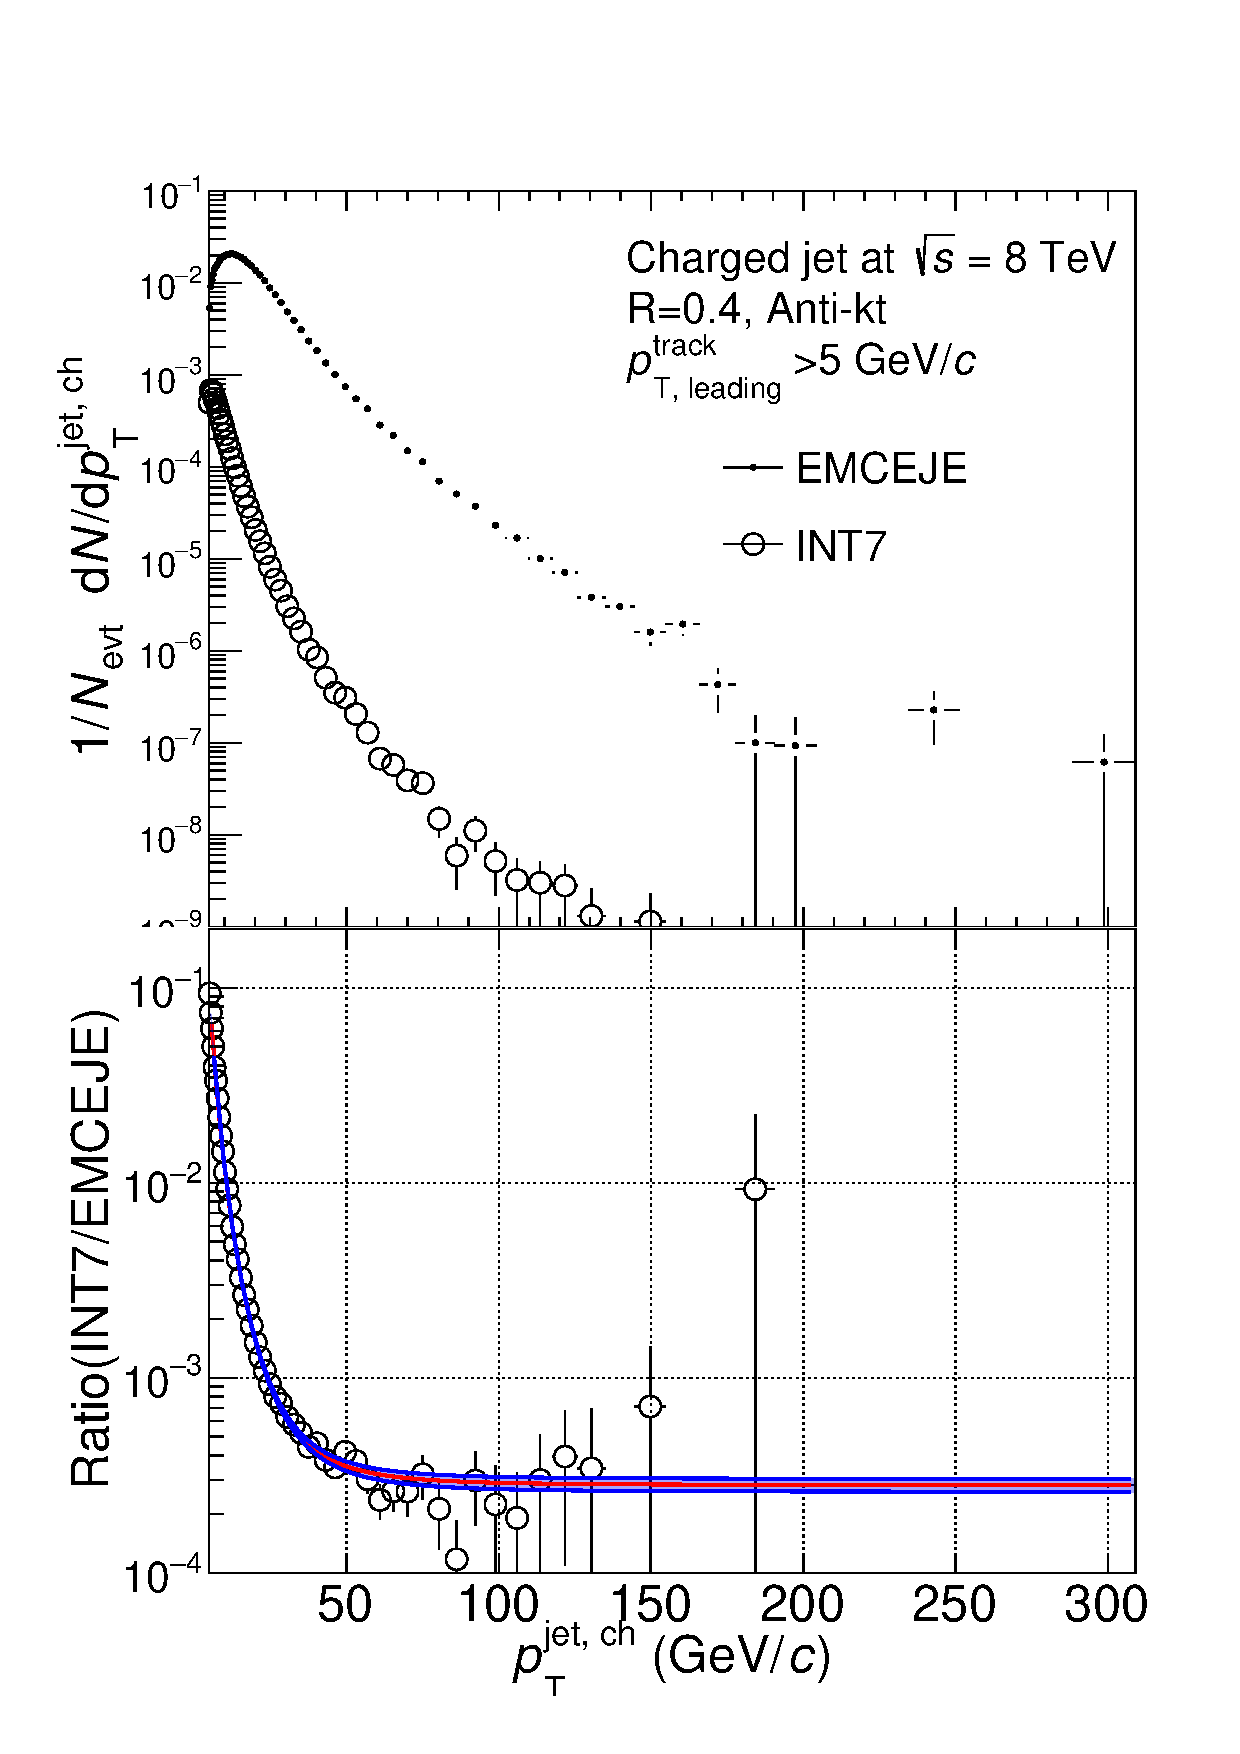
\includegraphics[width=1\linewidth]{JetToINT7TriggEff8TeV}\\
\column{.5\textwidth}
\begin{itemize}
  \item{Ratio shows \\ $\frac{\frac{1}{N_\mathrm{evt}^\mathrm{INT7}} \frac{\mathrm{d}N}{\mathrm{d}p_\mathrm{T,raw}^\mathrm{jet,ch}}}{\frac{1}{N_\mathrm{evt}^\mathrm{EMCEJE}} \frac{\mathrm{d}N}{\mathrm{d}p_\mathrm{T,raw}^\mathrm{jet,ch}}}$}
	\item{Fitted with $\frac{A}{(B+x^4)^C}+D$}
	\item{95 $\%$ confidence-range \\- Shown with blue\\- Systematic uncertainty}
  \item{Fit function\\- when on-the-fly filling}
\end{itemize}
\end{columns}
\end{frame}


\begin{frame}
\frametitle{Unfolding - closure test}
Detector efficiency is corrected by the unfolding method
\begin{columns}[c]
\column{.5\textwidth}
\centering
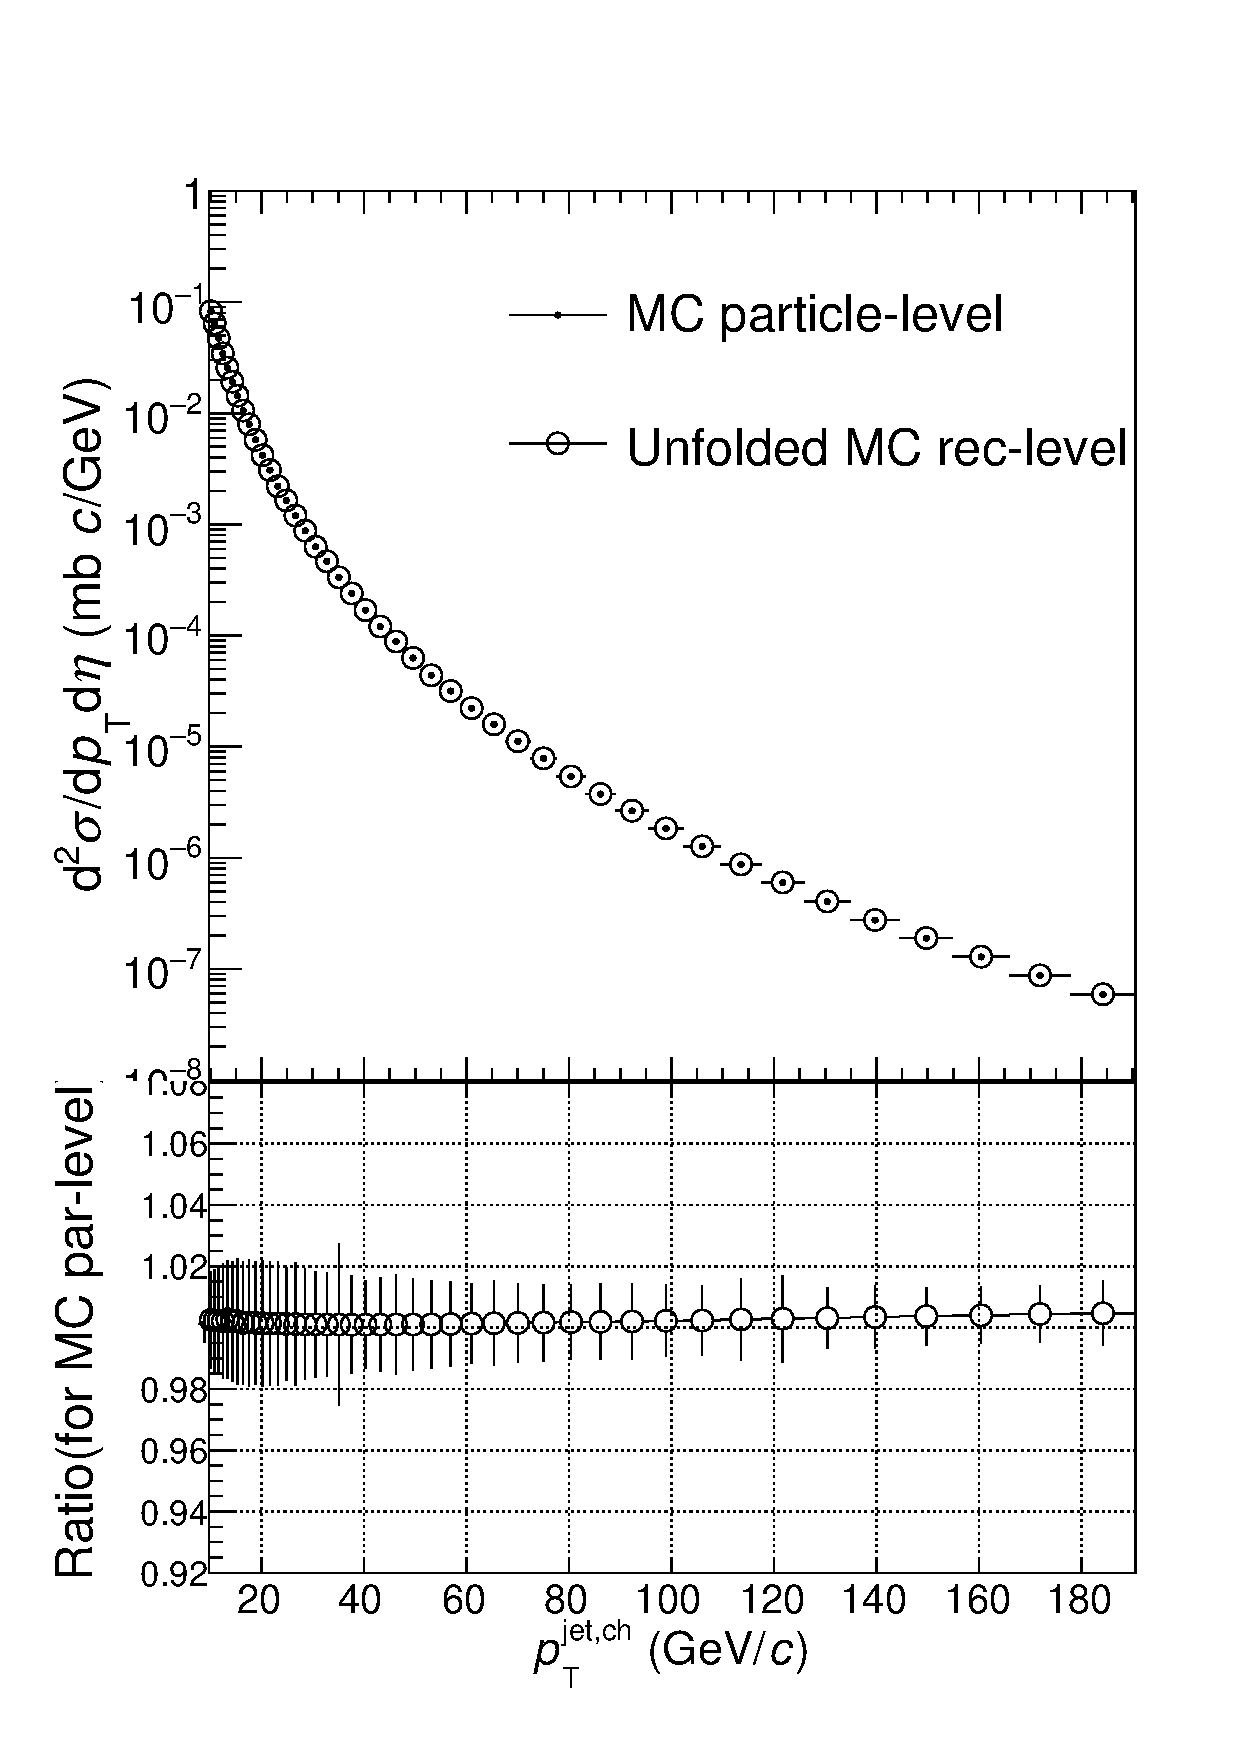
\includegraphics[width=1\linewidth]{jetpt_closure}\\
\column{.5\textwidth}
\begin{itemize}
  \small
	\item{Unfolding process\\$\frac{1}{N_\mathrm{evt}^\mathrm{EMCEJE}} \frac{\mathrm{d}N}{\mathrm{d}p_\mathrm{T,raw}^\mathrm{jet,ch}}$
  $\times$ $\frac{\frac{1}{N_\mathrm{evt}^\mathrm{INT7}} \frac{\mathrm{d}N}{\mathrm{d}p_\mathrm{T,raw}^\mathrm{jet,ch}}}{\frac{1}{N_\mathrm{evt}^\mathrm{EMCEJE}} \frac{\mathrm{d}N}{\mathrm{d}p_\mathrm{T,raw}^\mathrm{jet,ch}}}$
  \\ $\times$ $\mathcal{R}^{-1}(\frac{1}{N_\mathrm{evt}^\mathrm{mcrec}} \frac{\mathrm{d}N}{\mathrm{d}p_\mathrm{T,mcrec}^\mathrm{jet,ch}},\frac{1}{N_\mathrm{evt}^\mathrm{mcgen}} \frac{\mathrm{d}N}{\mathrm{d}p_\mathrm{T,mcgen}^\mathrm{jet,ch}})$}
  \normalsize
  \item{Package : RooUnfold}
	\item{Algorithm : Iterative(Bayesian)}
	\item{Regularization parameter : 4}
\end{itemize}
\end{columns}
\end{frame}


\begin{frame}
\frametitle{Final result}
\begin{columns}[c]
\column{.5\textwidth}
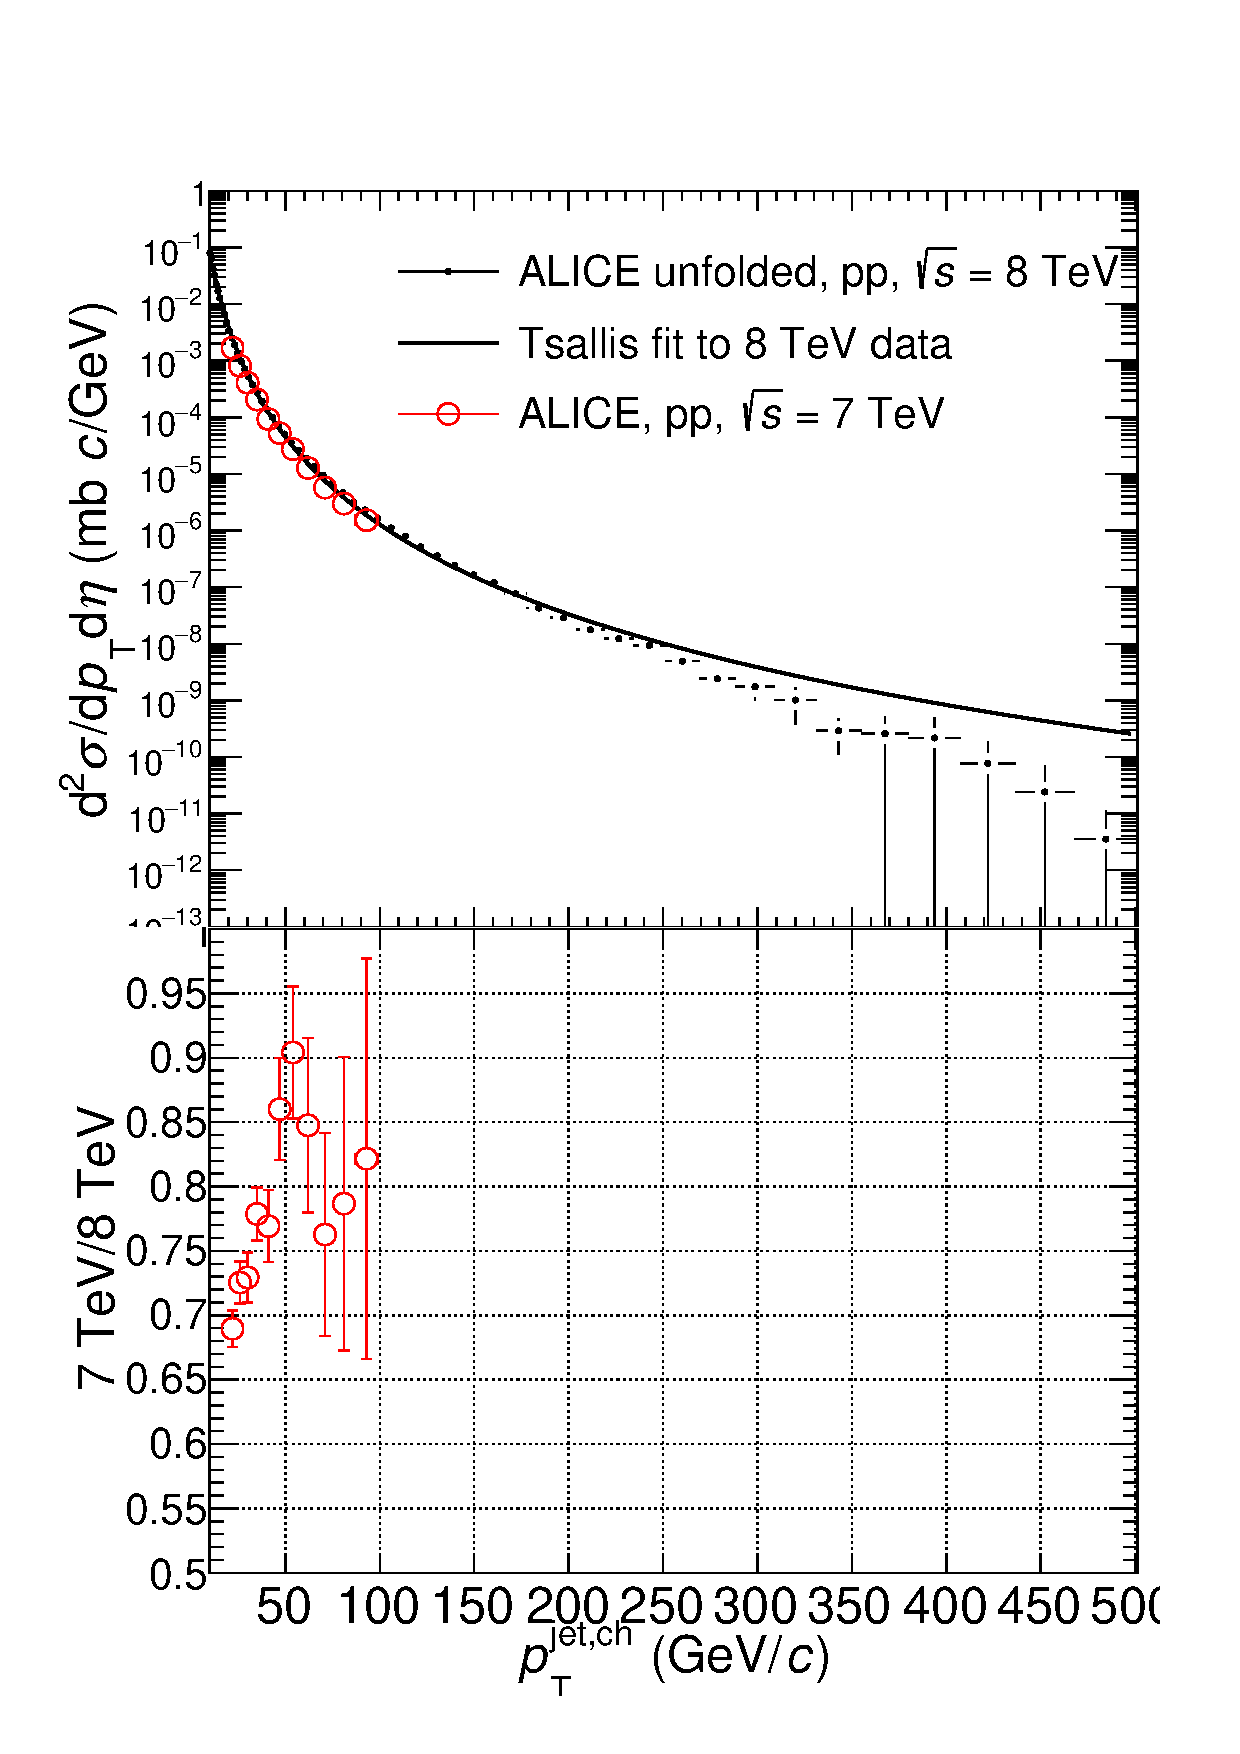
\includegraphics[width=1\linewidth]{jetpt_data_data.pdf}
\column{.5\textwidth}
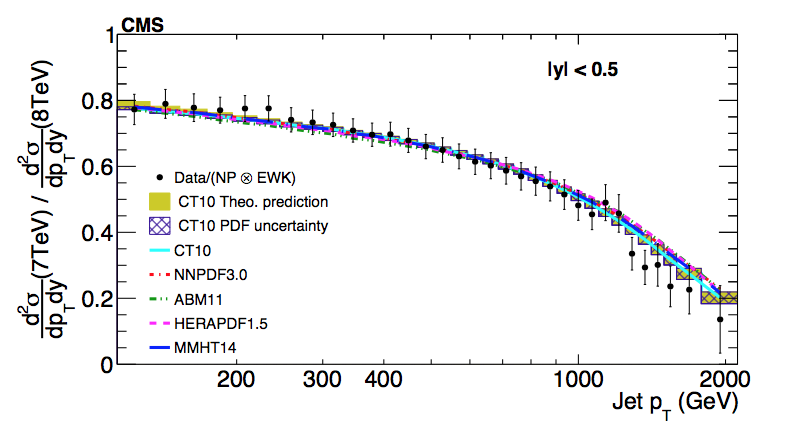
\includegraphics[width=1\linewidth]{CMSratio}\\
Ratio of CMS full jet spectra beteen 7 and 8 TeV$^{[1]}$
\begin{itemize}
  \item{around 0.8}
  \item{support the new 8 TeV result}
\end{itemize}
The new 8 TeV result extends to 300 GeV/$c$ (7 TeV, 100 GeV/$c$)
\end{columns}
\footnotetext[1]{arXiv:1609.05331v2 [hep-ex] 4 Apr 2017}
\end{frame}

\begin{frame}
\frametitle{Final result v.s models}
\begin{columns}[c]
\column{.5\textwidth}
\centering
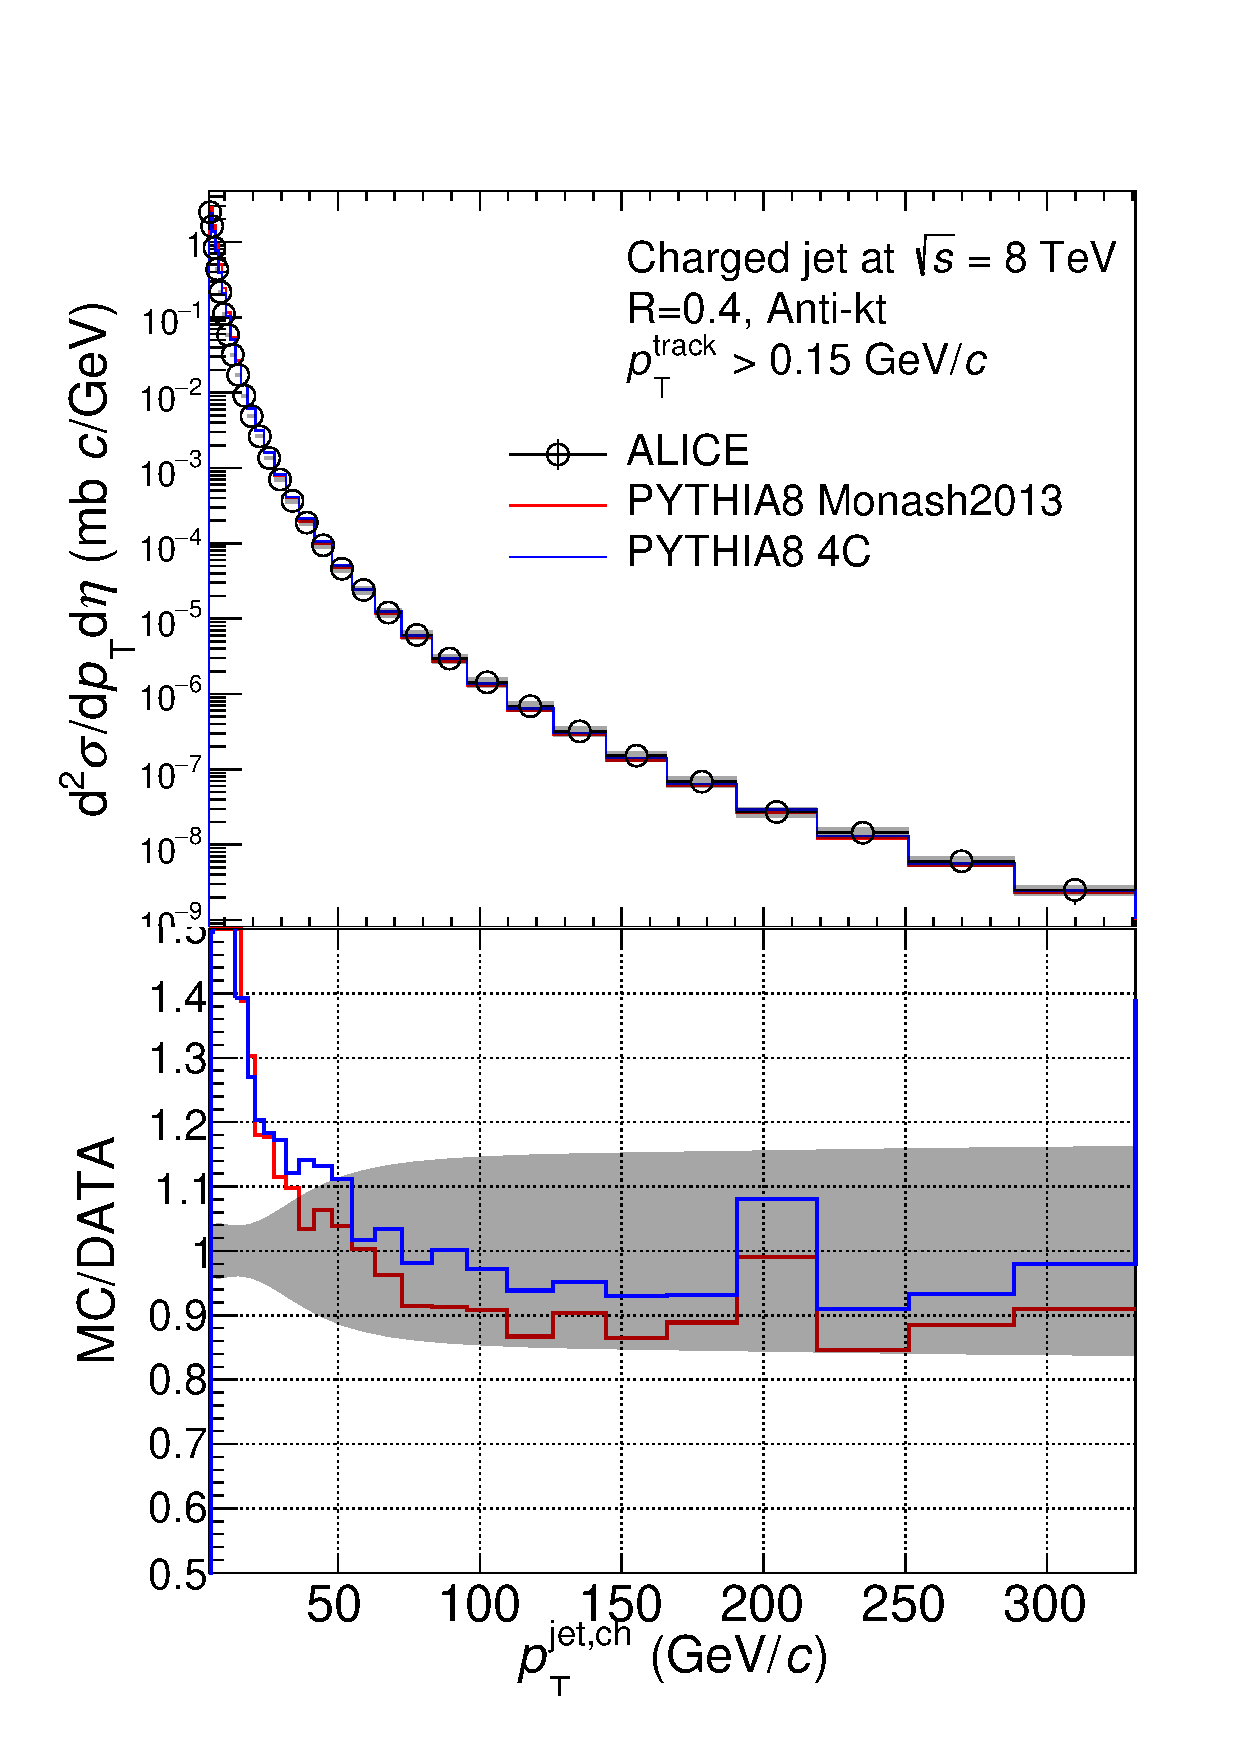
\includegraphics[width=1\linewidth]{jetpt8tev}\\
\column{.5\textwidth}
Systematic uncertainty
\begin{itemize}
  \item{Jet to INT7 trigger scaling : 10 $\%$}
  \item{INT7 to INEL normalisation : 2.95$\%$ \\(0.7718$\pm$0.0228 (2.95$\%$))}
  \item{Unfolding : 3 $\%$ }
\end{itemize}

\end{columns}
\end{frame}

%\begin{frame}
%\frametitle{Scaling to 5.02 TeV}
%pp results should be scaled to 5 TeV \\ to compare with 5 TeV p-Pb and Pb-Pb results
%\begin{columns}[t]
%\column{.5\textwidth}
%\centering
%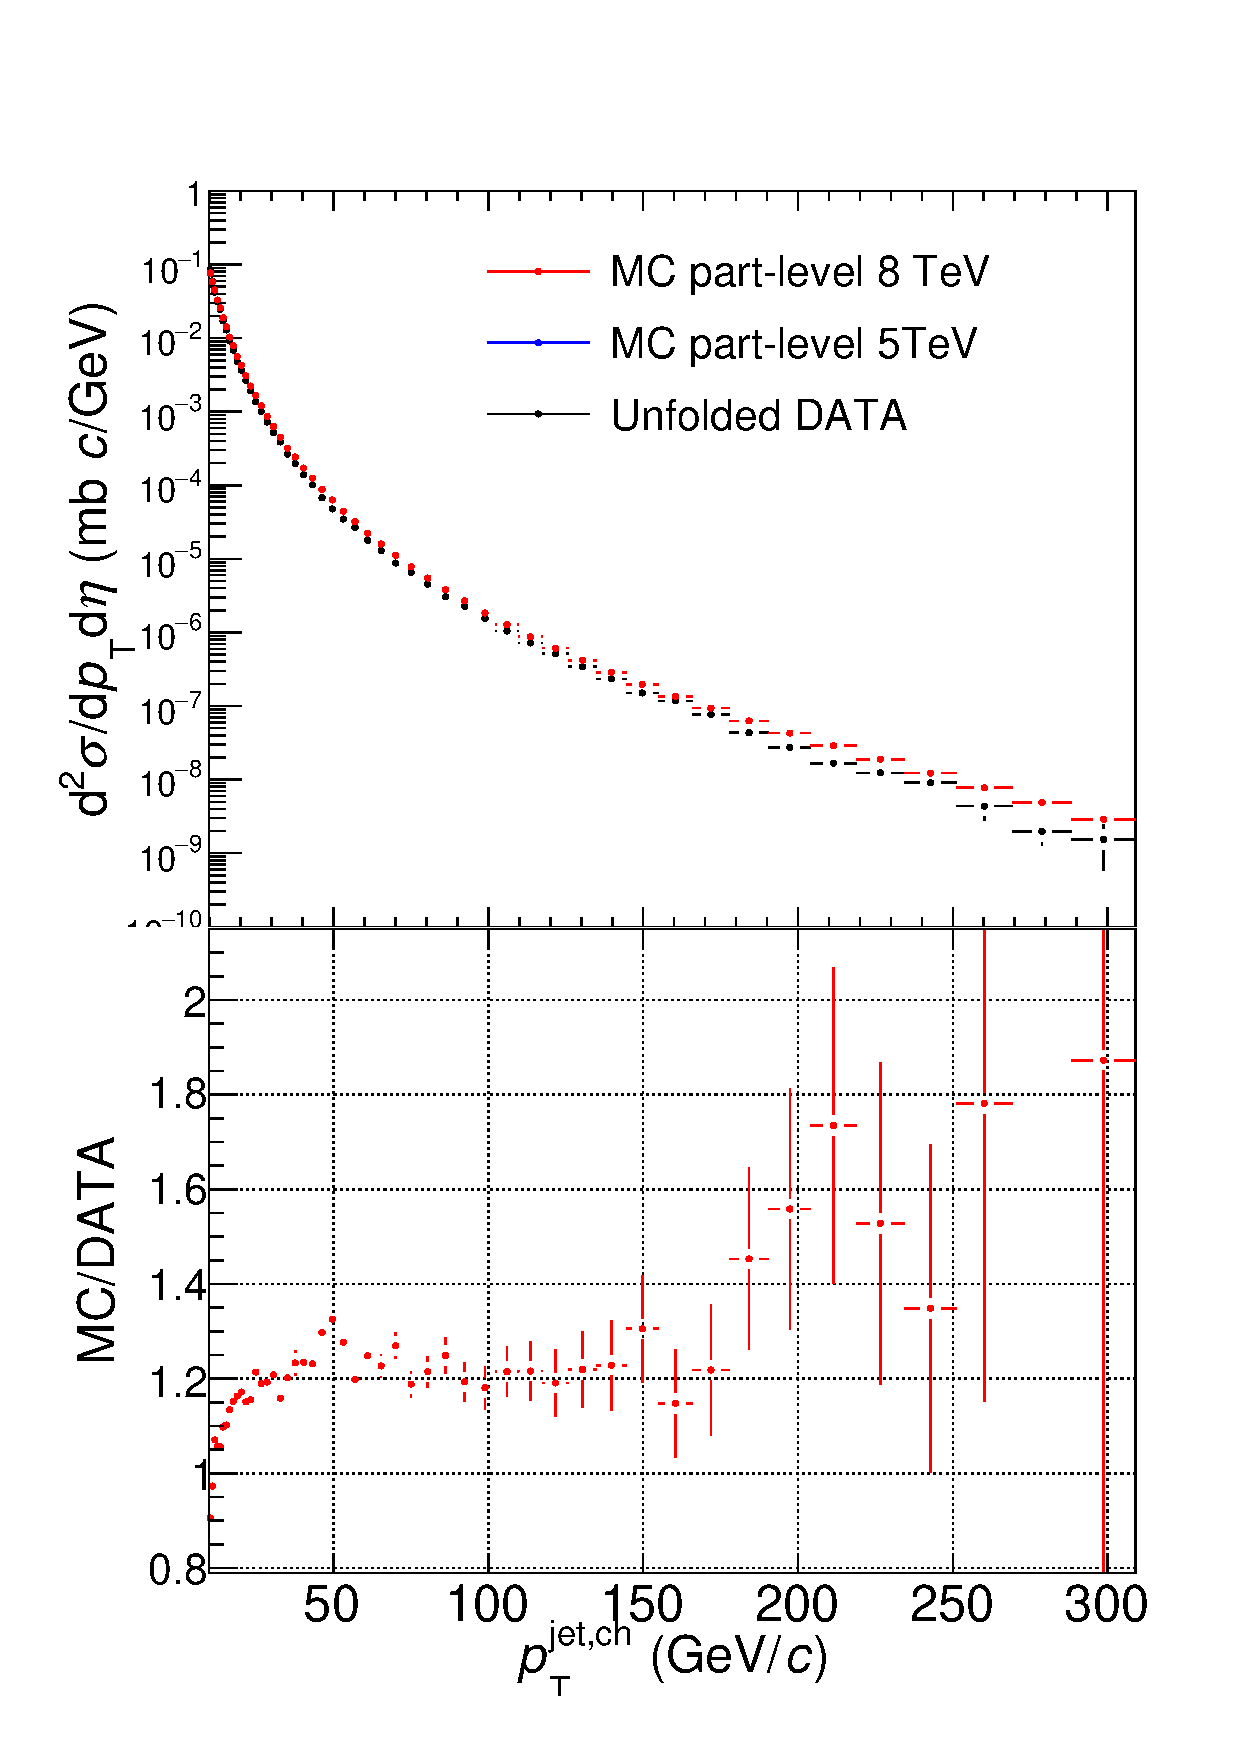
\includegraphics[width=1\linewidth]{jetpt_data_mc}\\
%\column{.5\textwidth}
%\end{columns}
%\end{frame}
